\documentclass[convert = false, tikz]{standalone}
\usepackage[utf8]{inputenc}
\usepackage{tikz}
\usepackage{adjustbox}
\usepackage{cancel}
\usetikzlibrary{automata, positioning, arrows, fit}
 
% arara: pdflatex
% arara: latexmk: { clean: partial }
\begin{document}
    
    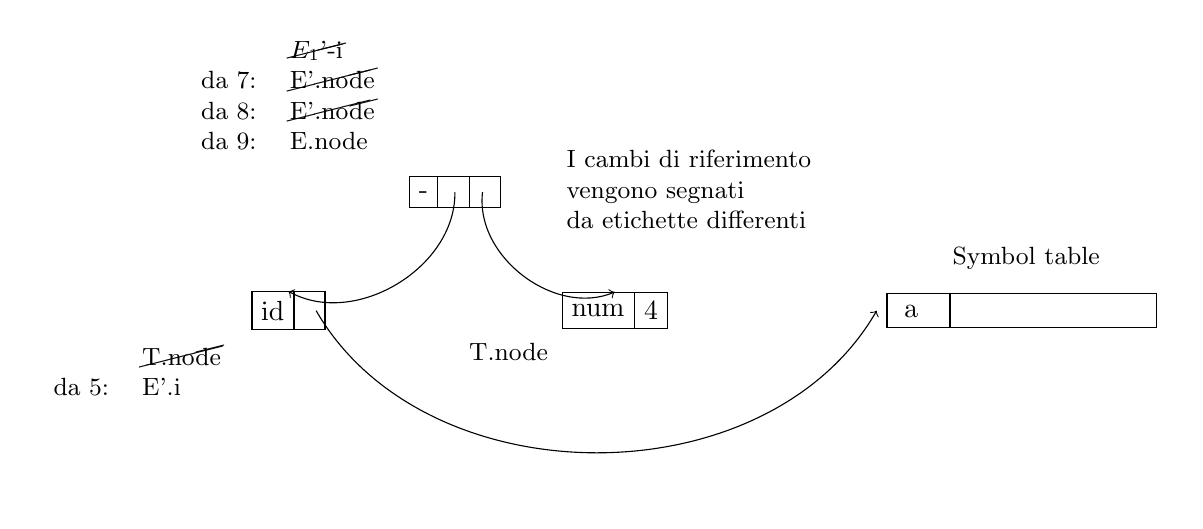
\begin{tikzpicture}[node distance=7cm, auto]

        % Disegna il primo nodo
        \node[draw, rectangle split, rectangle split parts=2, rectangle split horizontal] (first_node) {id \nodepart{second} };

        % Disegna il secondo nodo
        \node[draw, rectangle split, rectangle split parts=2, rectangle split horizontal, right=3cm of first_node] (second_node) {num \nodepart{second} 4};
        
        % Terzo nodo
        \node[draw, rectangle split, rectangle split parts=3, rectangle split horizontal, above right=1.5cm of first_node] (third_node) {- \nodepart{second} \nodepart{third} };

        % Definisci una coordinata, al centro della metà destra del primo nodo
        \coordinate (start) at ([xshift=1em]first_node.center);

        % Coordinate terzo nodo
        \coordinate (third_mid) at (third_node.center);
        \coordinate (third_right) at ([xshift=1em]third_node.center);

        % Disegna la tabella
        \node[right=of first_node, align=center] (table) {
            \begin{tabular}{|p{0.03\textwidth}|p{0.18\textwidth}|}
                \hline
                a & \\ \hline
            \end{tabular}
        };

        % Disegna la freccia
        \draw[->, bend right=60] (start) to (table.west);

        % Frecce terzo nodo
        \draw[->, bend left=60] (third_mid) to (first_node.north);
        \draw[->, bend right=60] (third_right) to (second_node.north);

        % Aggiungi le etichette testuali
        \node[below left=0.05cm and 0.05cm of first_node] {\small \begin{tabular}{ll} & \cancel{T.node} \\ da 5: & E'.i\end{tabular}};
        \node[below left=0.05cm and 0.05cm of second_node] {\small T.node};
        \node[above=0.05cm of table] {\small Symbol table};
        \node[above left=0.1cm and 0.1cm of third_node] {\small \begin{tabular}{ll} & \cancel{$E_1$'-i} \\ da 7: & \cancel{E'.node} \\ da 8: & \cancel{E'.node} \\ da 9: & E.node\end{tabular}};
        \node[right=0.5cm of third_node] {\small \begin{tabular}{l} I cambi di riferimento \\ vengono segnati \\ da etichette differenti \end{tabular}};
    \end{tikzpicture}

\end{document}